\begin{abstract}
A Mixture-of-Experts model too large for one consumer GPU keeps most of its experts in host memory, and decoding one
token at a time then waits on host reads. We ask how fast such decoding could be on a given machine, where the rest of
the time goes, and what knowing the future routing is worth. Two lower bounds follow from the fewest host reads any
cache of $C$ experts per layer can make (Belady's MIN with bypass) and the machine's measured read rates. On
\slAllMachines{} rented RTX 5090 machines, our llama.cpp expert cache takes the GPU's profiled compute plus its host
reads at the machine's best rate, with nothing fitted; its gap to the bound is that serialisation plus the reads MIN
would not make. Oracles inside the engine show that foresight pays when spent as MIN spends it, and that among MIN's
equally good schedules the one with the fewest admissions also wins where the PCIe link is slow. %%106-ABSTRACT
Half of MIN's saving over admitting every miss needs the routing of about \dcMed$\,C$ distinct experts per layer ahead,
which no forecaster we tested approaches.
\end{abstract}
]
\printAffiliationsAndNotice{}

\section{Introduction}
Open-weight Mixture-of-Experts (MoE) models now carry 30--120\,B parameters and activate a few billion per token; a
desktop GPU has 24--32\,GB. Running such a model for one user therefore means keeping most experts in host DRAM. Each
decoded token reads its routed experts from GPU memory if they are resident, and otherwise from host memory: either the
CPU runs the expert, or the expert is copied over PCIe into a GPU slot \citep{ivanov2021datamovement,hoefler2021sparsity}.
Many systems build on this: GPU expert caches \citep{eliseev2023offloading,xue2024moeinfinity,song2024promoe}, CPU
execution of misses \citep{kamahori2024fiddler,ktransformers,zhong2025hybrimoe}, a per-miss choice between the
two \citep{freetoken,dali2026} and expert prediction \citep{hwang2024pregated,zhu2025preattention,wang2026seqmoe}. Each
reports a speed-up over a baseline of its choosing. None states how fast the same machine \emph{could} decode the model
within the same GPU memory, or what the rest of the time is made of. We answer three questions for batch-1 decode of
gpt-oss-120b \citep{openai2025gptoss} and Qwen3-30B-A3B \citep{yang2025qwen3} on rented RTX 5090 hosts.

\textbf{How fast could it be?} (\cref{sec:limit}) No cache holding $C$ experts per layer reads fewer experts from host
memory than Belady's MIN with bypass. Those reads at the machine's measured read rate bound the time per token of any
system; a system that reads an expert only once its router has chosen it also pays the GPU's own compute in series,
which gives a tighter bound for every system we know of. The read time of both bounds is nearly reachable: a
microbenchmark that replays MIN's reads reaches \jdLayerMin--\jdLayerMax\% of it.

\textbf{Where does the time go?} (\cref{sec:gap}, \cref{fig:decomp}) Our cache's time per token is the GPU's profiled
compute plus its counted host reads at the machine's best rate, with nothing fitted. %%106-INTRO-LAW
Its gap to the bound therefore has two parts: the GPU's compute, which runs in series with the reads, and the reads it
makes beyond MIN's.

\textbf{What is knowing the future worth?} (\cref{sec:foresight,sec:horizon}) Oracles of the future routing built into the
engine show that foresight pays when it is spent as MIN spends it, caching MIN's set and reading each expert once:
\fxFetchAllGainMin--\fxFetchAllGainMax\% faster than our deployed cache on three hosts at six budgets. Which of MIN's
many equally good schedules is followed matters: the greedy one admits so often that it loses where the link is slow,
while the one with the fewest admissions gains on every machine it ran on. %%106-INTRO-ONLINE
Foresight also has a price: half of MIN's saving needs the routing of about \dcMed$\,C$ distinct experts per layer
ahead, which no online policy, learned admission order, speculative batch or forecaster we tested approaches.

\paragraph{Contributions.}
\begin{itemize}\setlength\itemsep{1pt}
\item \textbf{Two bounds on time per token} for exact-routing systems with $C$ slots per layer, from MIN's host reads
and the machine's probed rates, with evidence that their read time is nearly reachable (\cref{sec:limit}).
\item \textbf{A relation with nothing fitted} for where the time goes, found on \slLaunches{} launches and tested, with
its predictions committed before the runs, on new machines and a second model (\cref{sec:gap}).
\item \textbf{An in-engine study of what foresight is worth} and how it must be spent, on \slAllMachines{} machines,
including MIN's fewest-admission schedule and an online rule that carries its lesson (\cref{sec:foresight}).
\item \textbf{A price on foresight}: its value by horizon and accuracy, and a one-constant rule for the horizon in
distinct experts across nine models (\cref{sec:horizon}).
\item An artifact in which every prediction was committed before the machine it concerns started, and every number is
generated by a script (\cref{app:prereg,app:artifact}).
\end{itemize}

\section{Setting}\label{sec:setting}
\paragraph{Models and workload.} gpt-oss-120b (36 MoE layers of 128 experts, top-4, MXFP4, 13.25\,MB per expert) and
Qwen3-30B-A3B in BF16 (48 layers of 128 experts, top-8, 9.44\,MB per expert), on the 30 AIME-25 problems; the cache
carries over between problems, as in one user's session. The system comparison decodes 256 tokens per problem
greedily through each system's server. Everything else replays each model's own greedy output teacher-forced, so that
every configuration sees the same routing. A \emph{budget} is the share $C/E$ of each layer's experts that fit in GPU
slots: 11\%, 25\% and 40\% for gpt-oss, 12.5\%, 25\% and 43.75\% for Qwen3.

\paragraph{The engine.} Our cache is a 3{,}500-line patch to llama.cpp \citep{llamacpp}. Each MoE layer has $C$ GPU
slots. Routing is decided on the GPU, and resident experts run there. A \emph{miss} is read from host memory in one of
two ways: CPU helper threads run it, or it is \emph{fetched}, copied into a slot over PCIe and run on the GPU in the same
step. A per-machine table, computed from the machine's bandwidth probe, sets how many of a layer's misses to fetch. The
\emph{deployed} policy admits a miss into a slot when its decayed request count (half-life 16 tokens) beats the lowest
resident's by a margin $\kappa{=}1$; the CPU serves the admitted miss and a background copy then fills its slot, so the
expert is read from host memory twice.

\paragraph{Terms.} \emph{MIN} is Belady's optimum with bypass \citep{belady1966study,bypassopt}: it \emph{admits} a
miss only if some resident is needed later than the miss, and otherwise serves it without admitting it; this maximises
hits under $C$ slots \citep{carlisle1995kcoloring,jain2016hawkeye}. MIN has many hit-optimal schedules: the
\emph{greedy} one admits whenever it may; the \emph{fewest-admission} one admits as rarely as any schedule with the
most hits. An admitted expert is loaded \emph{in the step}, copied over PCIe before the GPU runs it (one host read, on
the critical path), or \emph{by the CPU}, served there and copied in the background (two reads). The oracles read the
routing of the rest of the problem from a trace recorded on the same machine; they decide, they do not predict
(\cref{tab:configs}). A budget is \emph{host-bound} when host reads, not the GPU, bound the time; the two smallest
budgets of each model are. Each host's probe measures how fast it reads its memory from CPU threads ($B_c$), over PCIe
($B_p$), and the highest rate by any method ($B_{\mathrm{host}}$); $B_p/B_c$ is its \emph{link-to-CPU ratio}.

\begin{table}[t]\centering\footnotesize
\caption{Cache configurations. \emph{Reads}: how many times an admitted expert is read from host memory. All run in the
same engine; the oracles read the future routing from a trace of the same text recorded on the same machine.}\label{tab:configs}
\setlength\tabcolsep{3pt}
\begin{tabular}{@{}p{0.27\linewidth}p{0.57\linewidth}c@{}}\toprule
Name & What it admits, and how & Reads \\\midrule
\multicolumn{3}{@{}l}{\emph{No foresight}} \\
deployed & decayed request count beats the lowest resident's by $\kappa{=}1$; the CPU serves the miss, then a background copy fills the slot & 2 \\
single read & the same admissions, fetched into the slot in the step & 1 \\
admit every miss & every miss fetched into the lowest-scored slot (demand fetch) & 1 \\
\midrule
\multicolumn{3}{@{}l}{\emph{Oracles}} \\
MIN, 2 reads & MIN with bypass (greedy rule); the CPU serves the miss, then a copy & 2 \\
MIN, 1 read & MIN with bypass (greedy rule); admissions fetched in the step & 1 \\
MIN, fewest adm. & the hit-optimal schedule with the fewest admissions (an LP per host), with 2 or 1 reads & 2 or 1 \\
MIN, prefetched & MIN, 1 read, plus copies issued three steps ahead & 1 \\
Belady & every expert of the coming steps, into the slot needed furthest ahead (also with 1 read, and prefetched) & 2 or 1 \\
window $W$ & admit every miss unless the next $W$ tokens show the victim needed sooner; victim the lowest-scored resident not seen in the window, else the one seen furthest & 1 \\
window $W$, recall $r$ & the same, each future expert kept with probability $r$, else replaced by a random one & 1 \\
deployed + window $W$ & the deployed policy with the same window and victim choice; the CPU serves the miss, then a background copy & 2 \\
\bottomrule
\end{tabular}
\end{table}


\paragraph{Statistics.} Time per token is averaged over problems; ratios are ratios of means paired by problem, with
95\% bootstrap intervals over problems. Machines differ far more than problems: two hosts with the same CPU model
differ by \pnSameCpuDiffMin--\pnSameCpuDiffMax\% in the deployed cache's time, while machines rented again came within
\jcRelaunchBaseMax\% of their first launch. The machine is therefore the unit: claims are about orderings that hold on
every machine of a stated class, pooled intervals resample machines and then problems \citep{kalibera2013rigorous}, and
the claims that rest on small effects carry intervals over repeated launches. Each job's predictions were committed
before its machine started; \cref{app:prereg} scores those of jobs 073 onward.

\section{Two Bounds on Time per Token}\label{sec:limit}
Consider any system that executes the model's exact routing with at most $C$ experts of each layer resident on the
GPU. Per token each of the $Lk$ routed experts is served by a resident copy or read from host memory, by the CPU that
runs it or by the copy that brings it into a slot. Let $R^\star$ be MIN's host reads per token, summed over layers, on
the routing trace; no policy, even one that knows the future, reads fewer. If $c$ experts per token run on the CPU,
host memory supplies at least $\max(R^\star,c)\,S$ bytes of experts of $S$ bytes each, and the GPU reads the dense
weights $D$ plus $(Lk-c)\,S$. With everything overlapped,
\begin{equation}
\bar T \;\ge\; \min_{0\le c\le Lk}\ \max\!\Big(\frac{D+(Lk-c)S}{B_{\mathrm{gpu}}},\ \frac{\max(R^\star\!,c)\,S}{B_{\mathrm{host}}}\Big).
\label{eq:limit}
\end{equation}
At a host-bound budget the minimum is at $c{=}0$ and the bound is MIN's read time, $R^\star S/B_{\mathrm{host}}$. The
bound covers exact routing, whole experts of unmodified bytes, at most $C$ residents per layer and one token per
forward pass; it drops all latencies and lets the two read paths share $B_{\mathrm{host}}$ freely. (Its MIN runs over
the problems in sequence and may evict an expert in the step that served it; the oracles restart at each problem and
keep each step's experts, which reads a few percent more.)

\paragraph{A tighter bound for systems that read on demand.} \Cref{eq:limit} overlaps the GPU's work with the host
reads. At batch size 1 a system that reads an expert only after its layer's router has chosen it cannot: layer $l$'s
misses are known only after layer $l$'s attention and router, and layer $l{+}1$ starts only after layer $l$'s experts.
Its time is at least the GPU's non-expert work plus the reads, in series:
\begin{equation}
\bar T_{\text{demand}} \;\ge\; T_{\text{GPU}} + \frac{R^\star S}{B_{\mathrm{host}}},
\label{eq:demand}
\end{equation}
where $T_{\text{GPU}}$, the GPU's attention, dense layers, norms and routers per token, is \slGneMin--\slGneMax\,ms for
gpt-oss in Nsight profiles of our engine on \slProfHosts{} hosts. Every system we compare reads on demand; only reading
before routing, that is foresight, can approach \cref{eq:limit}.

\paragraph{Where systems stand.} \Cref{tab:headline} places three systems against the bounds on two hosts. Our cache
leads FreeToken \citep{freetoken} at \bothLeadCells{} of \bothCells{} configurations and runs
\bothLlamaXMin--\bothLlamaXMax$\times$ stock llama.cpp at equal GPU expert memory; tuned over five settings on a third
host, FreeToken still trails at \fttLeadCells{} of six cells (\cref{app:system}). On the \slMachines{} machines of
\cref{sec:gap}, at gpt-oss 11\%, our cache stands at \slMaxEffLowMin--\slMaxEffLowMax\% of \cref{eq:limit} and at
\slDemEffLowMin--\slDemEffLowMax\% of \cref{eq:demand}. Scored by the same procedure at their papers' datasheet rates,
published batch-1 systems in the bound's class reach a median \audInclassMed\% of \cref{eq:limit} (\cref{app:audit}).

\begin{table*}[t]\centering\small
\caption{Decode speed at equal GPU expert memory on two RTX 5090 hosts. 30 AIME-25 problems, first 256 decode tokens,
greedy, session; our cache uses the FETCH split computed from each machine's bandwidth probe; FreeToken uses its faster
backend per budget, picked on listing B on a separate launch and carried over to the second host. Ratios are of mean
speeds, paired by problem, with 95\% bootstrap intervals. \emph{Speed limit}: the fastest any exact-routing system with
the same slots per layer can decode on that machine (\cref{sec:limit}: exact optimum, that host's highest probed rate,
datasheet GPU rate; \cref{tab:limit} tightens it). With every weight in the VRAM of an RTX PRO 6000 (the RTX 5090's
datasheet bandwidth, 96\,GB), stock llama.cpp decodes gpt-oss at 255 and Qwen3 at 178\,tok/s.
$^\dagger$Launch 1 for both systems: FreeToken's backend was picked on the launch it is scored on, which favours it,
and the row has no confirmation launch.}\label{tab:headline}
\resizebox{\textwidth}{!}{%
\begin{tabular}{llrrrcrrr}\toprule
Model & Experts & llama.cpp & FreeToken & Ours & Ours $\div$ FreeToken & Ours $\div$ & Speed & Ours, \% \\
 & on GPU & (tok/s) & (tok/s) & (tok/s) & (95\% CI) & llama.cpp & limit & of limit \\\midrule
\multicolumn{9}{l}{\textbf{Listing B}: Ryzen 9 9950X3D, card at 17001\,MHz memory clock, CPU 72\,GB/s, link 53, together 78} \\
gpt-oss-120b & 11\% & 34.9 & 54.0 {\scriptsize(hybrid)} & \textbf{69.9} & 1.294 [1.278, 1.312] & 2.00$\times$ & 172 & 41\% \\
gpt-oss-120b & 25\% & 40.0 & 85.6 {\scriptsize(hybrid)} & \textbf{109.2} & 1.275 [1.254, 1.295] & 2.73$\times$ & 430 & 25\% \\
gpt-oss-120b & 40\% & 47.7 & 132.2 {\scriptsize(offload)} & \textbf{152.5} & 1.154 [1.134, 1.172] & 3.20$\times$ & 519 & 29\% \\
Qwen3-30B-A3B & 12.5\% & 19.5 & 38.7 {\scriptsize(hybrid)} & \textbf{40.0} & 1.032 [1.022, 1.042] & 2.05$\times$ & 96 & 42\% \\
Qwen3-30B-A3B & 25\% & 22.1 & 54.7 {\scriptsize(hybrid)} & \textbf{63.1} & 1.153 [1.134, 1.173]$^\dagger$ & 2.86$\times$ & 214 & 30\% \\
Qwen3-30B-A3B & 43.75\% & 28.4 & 103.1 {\scriptsize(offload)} & \textbf{108.2} & 1.049 [1.036, 1.064] & 3.81$\times$ & 308 & 35\% \\
\midrule
\multicolumn{9}{l}{\textbf{Stock-clock host}: Ryzen 9 9950X, card at 14001\,MHz, CPU 56\,GB/s, link 53, together 66; FreeToken's backend carried over from listing B} \\
gpt-oss-120b & 11\% & 28.9 & 48.0 {\scriptsize(hybrid)} & \textbf{57.9} & 1.207 [1.195, 1.219] & 2.00$\times$ & 140 & 41\% \\
gpt-oss-120b & 25\% & 33.6 & 78.7 {\scriptsize(hybrid)} & \textbf{94.1} & 1.196 [1.163, 1.224] & 2.80$\times$ & 351 & 27\% \\
gpt-oss-120b & 40\% & 40.1 & 122.2 {\scriptsize(offload)} & \textbf{133.6} & 1.093 [1.077, 1.111] & 3.34$\times$ & 514 & 26\% \\
Qwen3-30B-A3B & 12.5\% & 16.1 & 32.7 {\scriptsize(hybrid)} & \textbf{33.5} & 1.027 [1.018, 1.036] & 2.08$\times$ & 78 & 43\% \\
Qwen3-30B-A3B & 25\% & 18.5 & 51.4 {\scriptsize(hybrid)} & \textbf{53.9} & 1.048 [1.037, 1.059] & 2.91$\times$ & 174 & 31\% \\
Qwen3-30B-A3B & 43.75\% & 23.8 & \textbf{98.3} {\scriptsize(offload)} & 95.8 & 0.974 [0.962, 0.987] & 4.02$\times$ & 305 & 31\% \\
\bottomrule\end{tabular}}\end{table*}


\paragraph{The read time is nearly reachable.} A microbenchmark (job 102) replays MIN's per-layer reads of gpt-oss at
11\% and 25\% on three hosts without the model, CPU threads reading part of each layer's experts while the copy engine
copies the rest into slots; waiting for every layer, it reaches \jdLayerMin--\jdLayerMax\% of the bound's read time
(\cref{tab:readsched}). An expert that is admitted and read once must cross the link; among MIN's hit-optimal schedules
the fewest admissions any of them needs is \laAdmMinLow{} per token at gpt-oss 11\%, against \laAdmGreedyLow{} for the
greedy one, and sending those over the link at the probe's link rate raises the bound by at most \laOverLowMax\% at 11\%
and \laOverMidMax\% at 25\% (\texttt{scripts/linkaware.py}). The GPU term of \cref{eq:limit}, by contrast, is loose
(batch-1 decode reaches \gpuEffPctGpt\% of the datasheet rate), but it binds only at the largest budgets; relaxing every
assumption at once is in \cref{tab:limit}.

\section{Where the Seconds Go}\label{sec:gap}
\paragraph{Time is GPU compute plus host reads.} For the deployed cache, one relation with nothing fitted describes the
time per token: %%106-LAW-EQ
\begin{equation}
T \;=\; G + \frac{R\,S}{B_{\mathrm{host}}},
\label{eq:sum}
\end{equation}
with $R$ the host reads per token the engine counts (misses and admissions) and $G$ the GPU's own kernel time per
token, \slGprofMin--\slGprofMax\,ms in \slProfN{} Nsight profiles on \slProfHosts{} hosts. %%106-LAW-BODY

\begin{figure*}[t]\centering
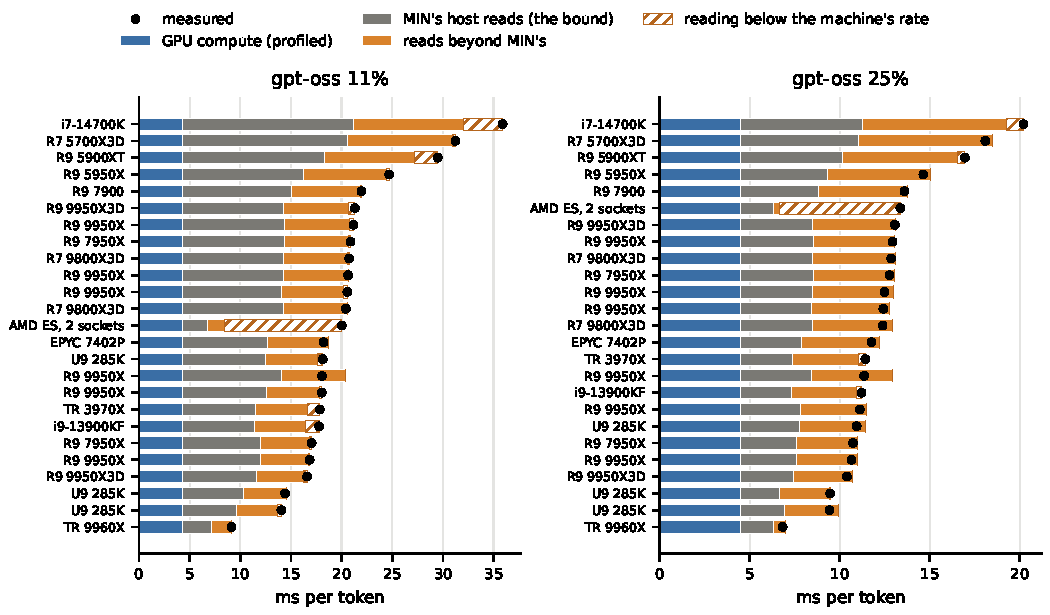
\includegraphics[width=\textwidth]{figs/decomp.pdf}
\caption{Where the seconds go, machine by machine: the deployed cache's time per token at the two host-bound gpt-oss
budgets split by \cref{eq:sum} into the GPU's own compute (the median of the profiles at that budget), MIN's host
reads at the machine's best rate (the bound of \cref{eq:limit}) and the reads the cache makes beyond MIN's; the dot is
the measured time. One launch per machine (\dcMachinesLow{} machines). Nothing is fitted: $G$ comes from profiles,
the reads from the engine's counters and the rate from each machine's probe.}
\label{fig:decomp}
\end{figure*}

\section{What Knowing the Future Is Worth}\label{sec:foresight}
The deployed cache does not know which experts the coming tokens will need. Oracles that read the future routing from a
trace measure what that knowledge is worth and how it must be spent: on three hosts (O3--O5) at all six budgets, on a
\pnHosts-host panel at the two host-bound gpt-oss budgets, and on follow-up launches. A running example: on O4 (a Ryzen
9 9950X) at gpt-oss 11\%, \cref{eq:limit} gives \slExBoundMs\,ms per token and \cref{eq:demand} \slExDemandMs; the
deployed cache takes \fsExBaseMs, MIN copying each admission in the step \fsExFetchMs, and MIN with the copies made a few
steps ahead \fsExPacedMs.

\begin{figure*}[t]\centering
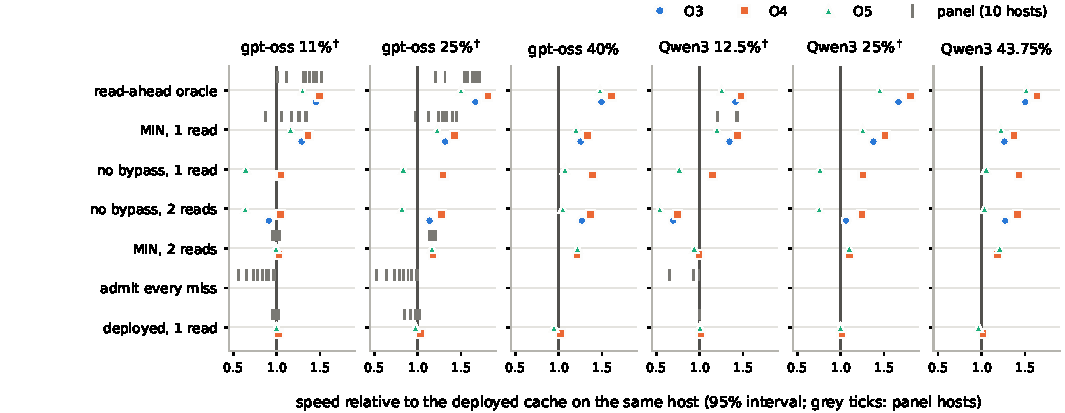
\includegraphics[width=\textwidth]{figs/factorial.pdf}
\caption{What foresight is worth in the engine, by how it is spent: speed of each configuration of \cref{tab:configs}
relative to the deployed cache on the same host, at the six budgets ($^\dagger$host-bound). Hosts O3, O4 and O5 at
every budget; the \pnHosts{} panel hosts (grey ticks) at the two gpt-oss host-bound budgets, and \pnHostsQlow{} of them
at Qwen3 12.5\%. Within-host 95\% intervals are mostly narrower than the markers. Admitting what MIN admits and reading
it once (\emph{MIN, 1 read}) gains at every budget on these hosts; the usual ways of spending foresight (\emph{Belady},
\emph{MIN, 2 reads}) gain at some budgets and lose at others.}
\label{fig:factorial}
\end{figure*}

\paragraph{Spent as MIN spends it, foresight pays.} MIN with each admission copied once, in the step, is faster than
the deployed cache at every budget on O3--O5, by \fxFetchAllGainMin--\fxFetchAllGainMax\%, and by
\fxPacedAllGainMin--\fxPacedAllGainMax\% with the copies made ahead (\cref{fig:factorial}). The usual ways of spending
foresight waste reads: Belady prefetch admits experts MIN would bypass, and serving a miss on the CPU before copying it
reads every admission twice. They read \fxUsualReadsOverOptMin--\fxUsualReadsOverOptMax$\times$ MIN's bytes and, at the
smallest budget of each model on O4 and O5, gain at most \fxUsualLowGainMax\% or lose; the trade-off is classical for
disks \citep{cao1995prefetching} and CPU caches \citep{jain2018prefetch}.

\paragraph{Which of MIN's schedules is followed matters.} The greedy schedule admits a miss whenever some resident is
needed later, and may evict it again before its next use; the fewest-admission schedule copies
\jfCopyRatioMin--\jfCopyRatioMax{} times as many experts in the step. Given to the engine on \jkLaunches{} launches on
\jkMachines{} machines (jobs 104--106), it gains over the deployed cache on every one
(\jkPlanMin--\jkPlanMax$\times$ at gpt-oss 11\%), and over the greedy schedule by \jkGainBalMin--\jkGainBalMax{} in
speed ratio on the \jkBalMachines{} machines whose link reads at \jkBalRatioMin--\jkBalRatioMax{} of their CPU rate. Where
the link reads at under a third of the CPU rate, the greedy schedule loses (\jkSlowFetchMin--\jkSlowFetchMax$\times$)
and the fewest-admission one gains (\jkSlowPlanMin--\jkSlowPlanMax$\times$); %%106-SLOW
Where the link is as fast as the CPU, copies in the step are cheap and the two schedules tie. Host by host, both loads
and both budgets are in \cref{app:more}.

\paragraph{The machine decides how much.} Across machines, the gain of every state that moves reads from the CPU to
the link follows the link-to-CPU ratio: for MIN copied in the step, Spearman \rcFetchRatio{} [\rcFetchRatioLo,
\rcFetchRatioHi] over \rcFetchRatioN{} machines (\cref{fig:hostdep}). Machines also differ more than problems: they
carry \ppVarHostsFetchMax\% of the variance of that state's log gain, problems \ppVarProbFetchMin--\ppVarProbFetchMax\%
(\cref{app:more}).

\begin{figure*}[t]\centering
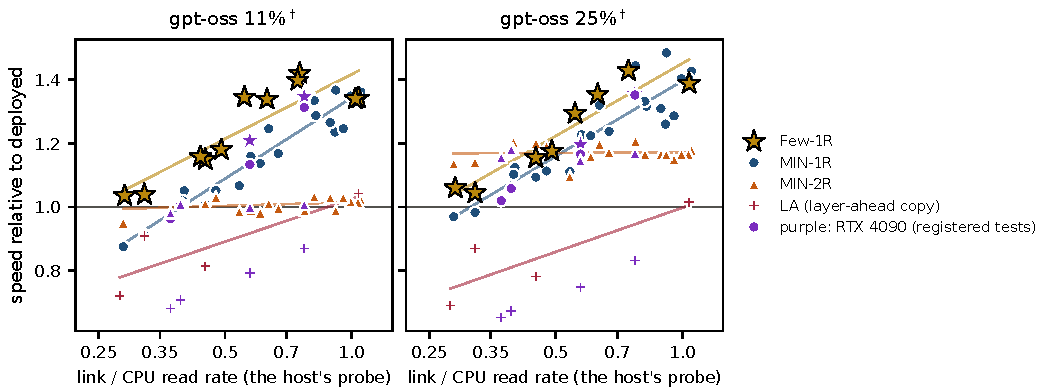
\includegraphics[width=\textwidth]{figs/hostdep.pdf}
\caption{Which way of spending foresight pays depends on the machine: speed relative to the deployed cache on the same
host against the host's link-to-CPU read-rate ratio from its own probe, at the two gpt-oss host-bound budgets. Stars:
MIN's fewest-admission set, copied in the step (jobs 104--106). Crosses: the deployed cache with the engine's
layer-ahead copy (job 105). Lines: least-squares fits in the log of the ratio, for the trend only.}
\label{fig:hostdep}
\end{figure*}

\paragraph{The lesson, carried online: admit less.} The fewest-admission schedule wins because an admission costs a
read. The deployed cache's admissions are second reads, so the lesson applies to it without foresight. %%106-ONLINE

\section{How Much Foresight Is Needed}\label{sec:horizon}
The oracles know the whole future; a forecaster would know part of it, imperfectly. We give the cache a
\emph{window}, the routing of the next $W$ tokens, exact or degraded (each future expert kept with probability $r$ and
replaced otherwise, so that precision and recall are both $r$), and ask what it is worth in the engine and, on nine
models' traces, how long it must be. The window policies and their engine runs are detailed in \cref{app:value}.

\paragraph{A short window pays little against the deployed cache.} Given to the deployed policy, so that it changes
only what is cached, a 16-token window runs \jaBSixteenLowMin--\jaBSixteenLowMax$\times$ the deployed cache at
gpt-oss 11\% on \jaHosts{} hosts, about what MIN with two reads gains; shorter or half-right windows lose up to
\jaWorstBLossPct\%. Measured against admitting every miss, the online policy that reads least at these budgets, windows
recover a share of MIN's gain quickly (\cref{fig:value}): exact windows of 4 and 16 tokens recover
\pnShareFourLowMin--\pnShareFourLowMax{} and \pnShareSixteenLowMin--\pnShareSixteenLowMax{} of it in time at gpt-oss
11\%. Accuracy matters as much as horizon: an 8-token window right half the time recovers
\pnShareEightHalfLowMin--\pnShareEightHalfLowMax, about what 2 exact tokens buy.

\begin{figure*}[t]\centering
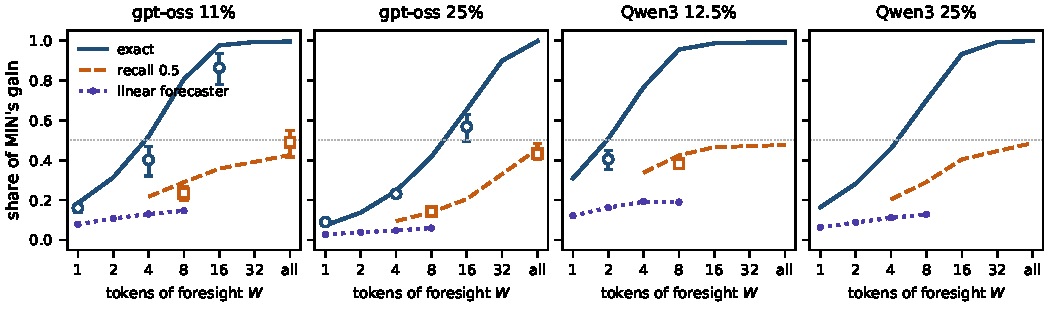
\includegraphics[width=\textwidth]{figs/value.pdf}
\caption{The value of partial foresight at the four host-bound budgets: the share of MIN's gain over \emph{admit every
miss} recovered by exact routing of the next $W$ tokens (solid), by a window whose experts are each right with
probability 0.5 (dashed), and by a linear forecaster fitted on other text (dotted), in host reads on the AIME routing
the engine runs; markers: the same share in time per token on the panel hosts (mean, and range over hosts; \pnHostsLow{} hosts
for gpt-oss, \pnHostsQlow{} for Qwen3 at 12.5\%; no Qwen3 run at 25\%). The grey line marks half of the gain.}
\label{fig:value}
\end{figure*}

\paragraph{The horizon is measured in distinct experts.} On nine models' own sampled text (33{,}000--152{,}000
tokens), the window $W_{50}$ that closes half of the read gap between admitting every miss and MIN ranges from
\dcWMin{} to \dcWMax{} tokens. Paging theory measures lookahead in distinct pages
\citep{albers1997lookahead,breslauer1995lookahead}, and so does the rule that fits: the experts a layer requests within
$W_{50}$ number about \dcMed$\,C$ (quartiles \dcLo--\dcHi). Given a model's routing trace, this one-constant rule
predicts its horizon as well as a two-constant power law in tokens (\cref{app:traces}). A forecaster's target is thus
the next $\approx$\dcMed$\,C$ distinct experts of each layer.

\paragraph{Nothing realisable reaches it.} Forecasters trained on routing histories, linear or recurrent, close at most
\lfShareMaxGpt\% of the read gap on gpt-oss: their precision falls with the horizon (\lfPrecOneGpt{} one token ahead,
\lfPrecFourGpt{} four ahead), and over a window they do no better than random errors of the same precision
(\cref{fig:value}, dotted). Speculative batches save an online cache \bkSameNineMin--\bkSameNineMax\% of its reads at
90\% draft acceptance and cost \bkSameEightLossMin--\bkSameEightLossMax\% at 80\% \citep{spmoe,moespac2026,cascade2025}.
Layer-ahead predictors \citep{hwang2024pregated,zhu2025preattention} reach \laRecallK\% recall in our engine but see less
than one token ahead, so they can only hide reads under the GPU's compute: the engine's layer-ahead copy, which copies
one predicted expert per layer ahead of use, gains \jgPfLowFastMin$\times$ where the link is as fast as the CPU and
loses elsewhere, down to \jgPfLowMin$\times$ (job 105, \cref{tab:job105}).

\section{Related Work}\label{sec:related}
\paragraph{Offloading systems.} Demand-paging systems cache experts per layer and copy misses over
PCIe \citep{eliseev2023offloading,xue2024moeinfinity,song2024promoe,tang2024hobbit,swapmoe2024,adapmoe2024,edgemoe2023,expertflow,pagingexperts2026},
or use predicted expert activations to decide what to keep \citep{sida2024}; an upstream
llama.cpp pull request adds such a cache, admitting every miss into an LRU \citep{llamacpppr29887}. CPU-execution
systems run non-resident experts on the host \citep{kamahori2024fiddler,ktransformers,zhong2025hybrimoe,daop2025,wang2026cloudgrade,atsinfer2026},
as PowerInfer runs a dense model's cold neurons \citep{powerinfer2024};
a set-associative GPU cache with CPU-executed misses \citep{huang2025cpugpu}, a llama.cpp fork \citep{leloch2026,llamacppdisc24528}
and two llama.cpp pull requests \citep{llamacpppr26563,llamacpppr27861} are the closest designs to ours.
FreeToken \citep{freetoken} and DALI \citep{dali2026} split each layer's misses between CPU and PCIe. Predictors guess
upcoming experts from the previous layer's state \citep{hwang2024pregated,zhu2025preattention}, several tokens ahead
with a learned forecaster \citep{wang2026seqmoe,mira2026}, or from draft tokens \citep{spmoe,moespac2026,cascade2025};
Read-ME decouples the router so routing is known in advance \citep{readme2024}. Batched-throughput
systems \citep{flexgen2023,cao2024moelightning,yuan2025moelens} and flash or SSD tiers \citep{llminflash2024,ssdllama,edgezero} are outside our
scope.

\paragraph{Bounds, oracles and caching theory.} WiSP \citep{wisp2026} bounds decode by PCIe turnover, Budgeting
Bytes \citep{budgetingbytes2026} by bytes over bandwidth for a given fetch set, and MoE-CAP \citep{moecap} measures
bandwidth utilisation against a single peak; the roofline \citep{williams2009roofline} is the single-memory ancestor of
our bound. \citet{zhang2026reproducible} proposes a trace-level evaluation contract and reports a 44--46\% gap
between causal policies and MIN with bypass; \citet{liang2026lrc} measure, across 20 models, the hit rate
of an oracle cache that sees $m$ tokens ahead against the cache ratio $C/k$. We add the time domain: an oracle inside a
real engine, the cost of how foresight is spent, and a horizon rule in distinct experts. SAEM \citep{saem2026}
gives its own stage-level planner perfect knowledge of the coming stage in its engine and finds that worth at most
about 14\% on an A100; SpecMD \citep{specmd} benchmarks expert-cache and speculative prefetch policies across hardware; \citet{angelopoulos2025cache} give competitive bounds for layered expert paging. With bypass, MIN maximises hits
exactly \citep{carlisle1995kcoloring,jain2016hawkeye}; when bypass and admission cost differ, the time-optimal placement
is a different problem \citep{bypassopt}, which is why we use MIN's reads as an input to a bound rather than as a
time-optimal policy. Choosing among hit-optimal schedules by what admissions cost has precedents: Demand-MIN for
prefetching \citep{jain2018prefetch}, offline-optimal caching as a min-cost flow over reuse
intervals \citep{berger2018foo}, and admission rationing in flash caches \citep{flashield2019}. Our fewest-admission
schedule is that interval formulation with admissions as a second objective, measured in an engine. Lookahead in paging is valuable when measured in distinct pages \citep{albers1997lookahead,breslauer1995lookahead},
and learning-augmented paging is most robust with predictions of whether a page will be evicted before its next
use \citep{antoniadis2023succinct}; learned replacement imitates Belady in CPU and content-delivery
caches \citep{jain2016hawkeye,song2020lrb} and in an SSD-backed expert cache \citep{flashmoe2026}.

\section{Limitations}\label{sec:limits}
%%LIMITS

\section{Conclusion}
%%CONCLUSION
